\begin{figure*}[!h]
    \centering
    \begin{minipage}{.5\textwidth}
        \centering
        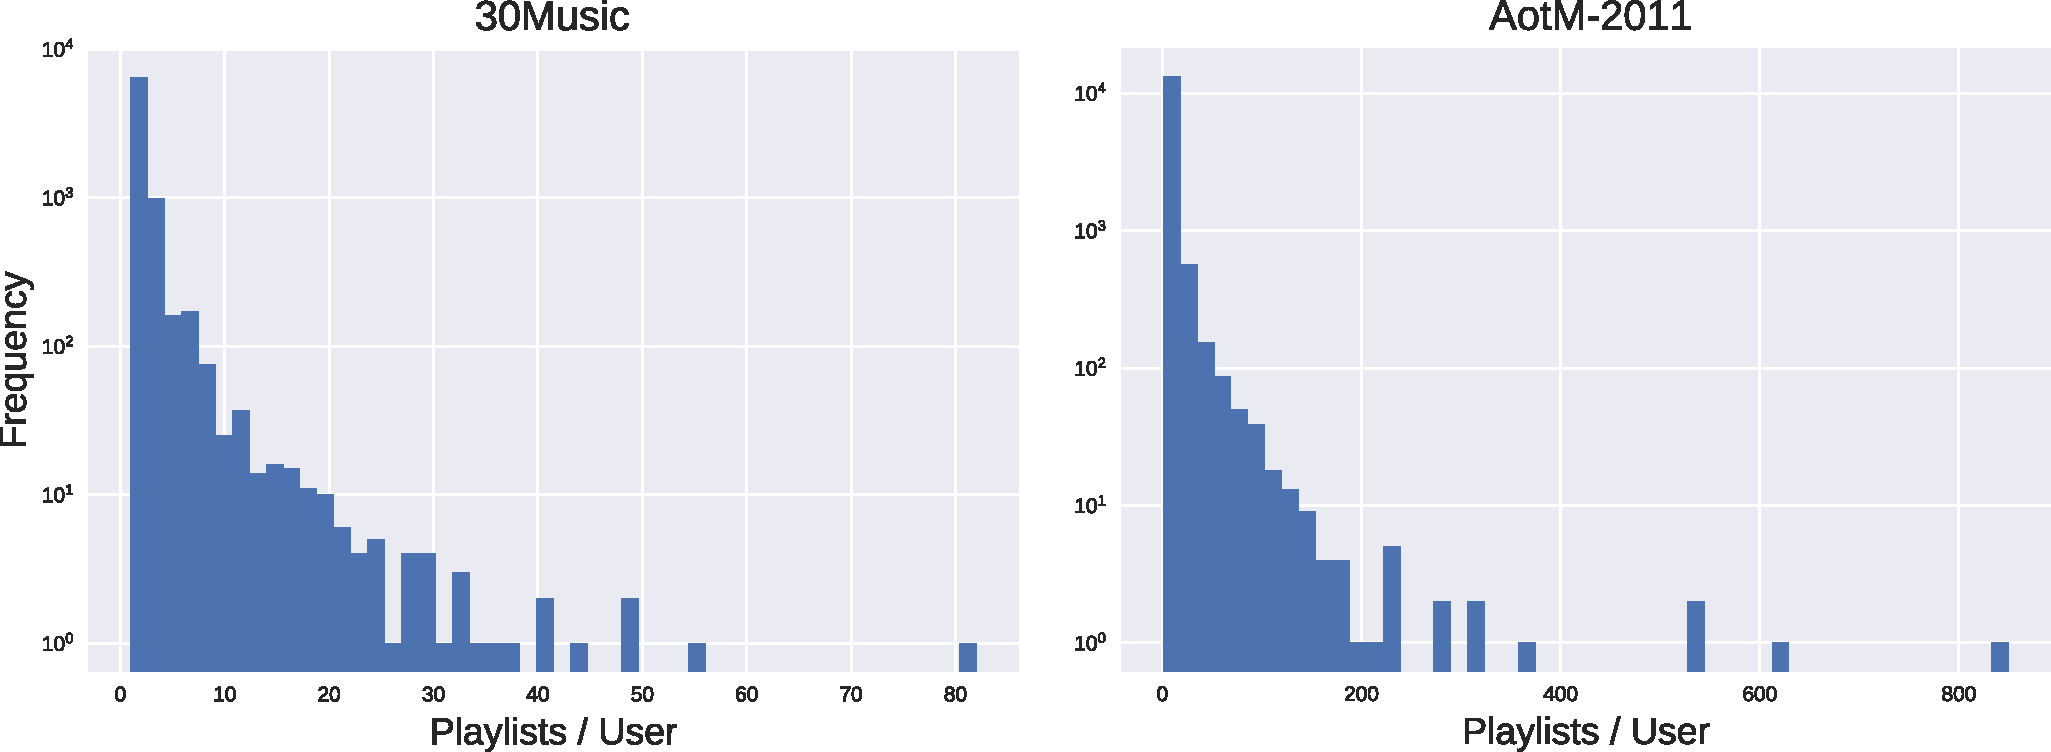
\includegraphics[width=.98\linewidth]{fig/hist_pluser.pdf}
        \caption{Histogram of the number of playlists per user}
        \label{fig:hist_pluser}
    \end{minipage}%
    \begin{minipage}{0.5\textwidth}
        \centering
        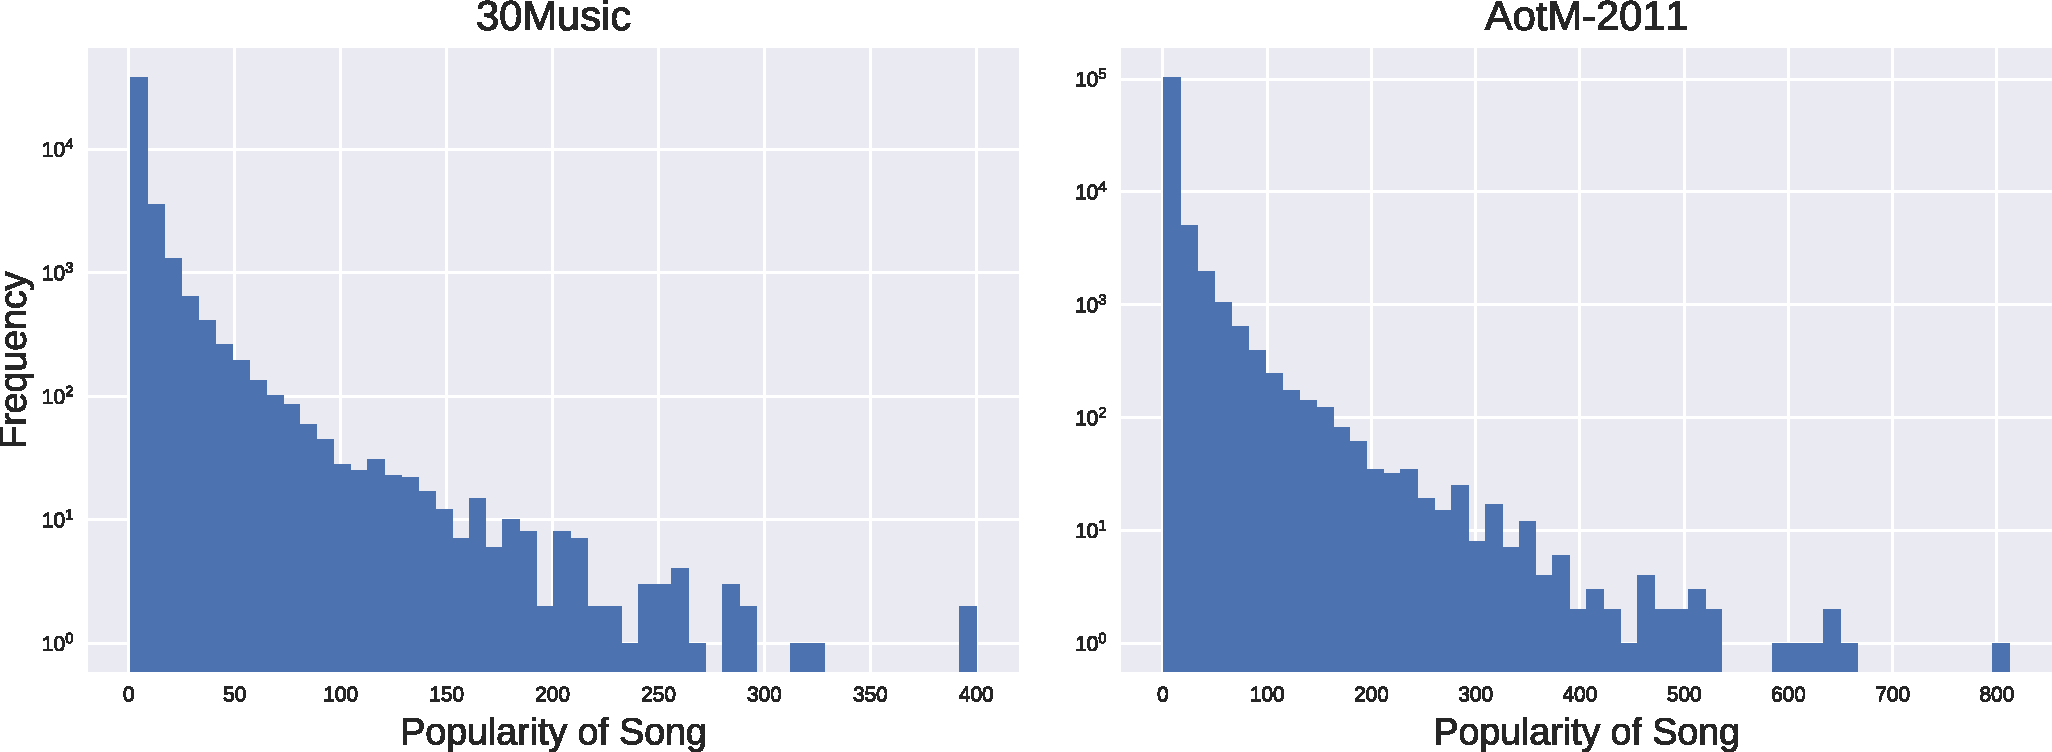
\includegraphics[width=.98\linewidth]{fig/hist_songpop.pdf}
        \caption{Histogram of song popularity}
        \label{fig:hist_songpop}
    \end{minipage}
\end{figure*}

The histograms of the number of playlists per user as well as song popularity 
(\ie the number of occurrences of a song in all playlists)
of the two datasets are shown in Figure~\ref{fig:hist_pluser} and Figure~\ref{fig:hist_songpop},
respectively.
We can see from Figure~\ref{fig:hist_pluser} and \ref{fig:hist_songpop} that both the number
of playlists per user and song popularity follow a long-tailed distribution, which imposes further challenge to the learning task 
as the amount of data is very limited for users (or songs) at the tail.
